
\exercise{Symmetry}{2}
Find at least 5 eigenvalues of the adjacency matrix of the following network:
\begin{center}
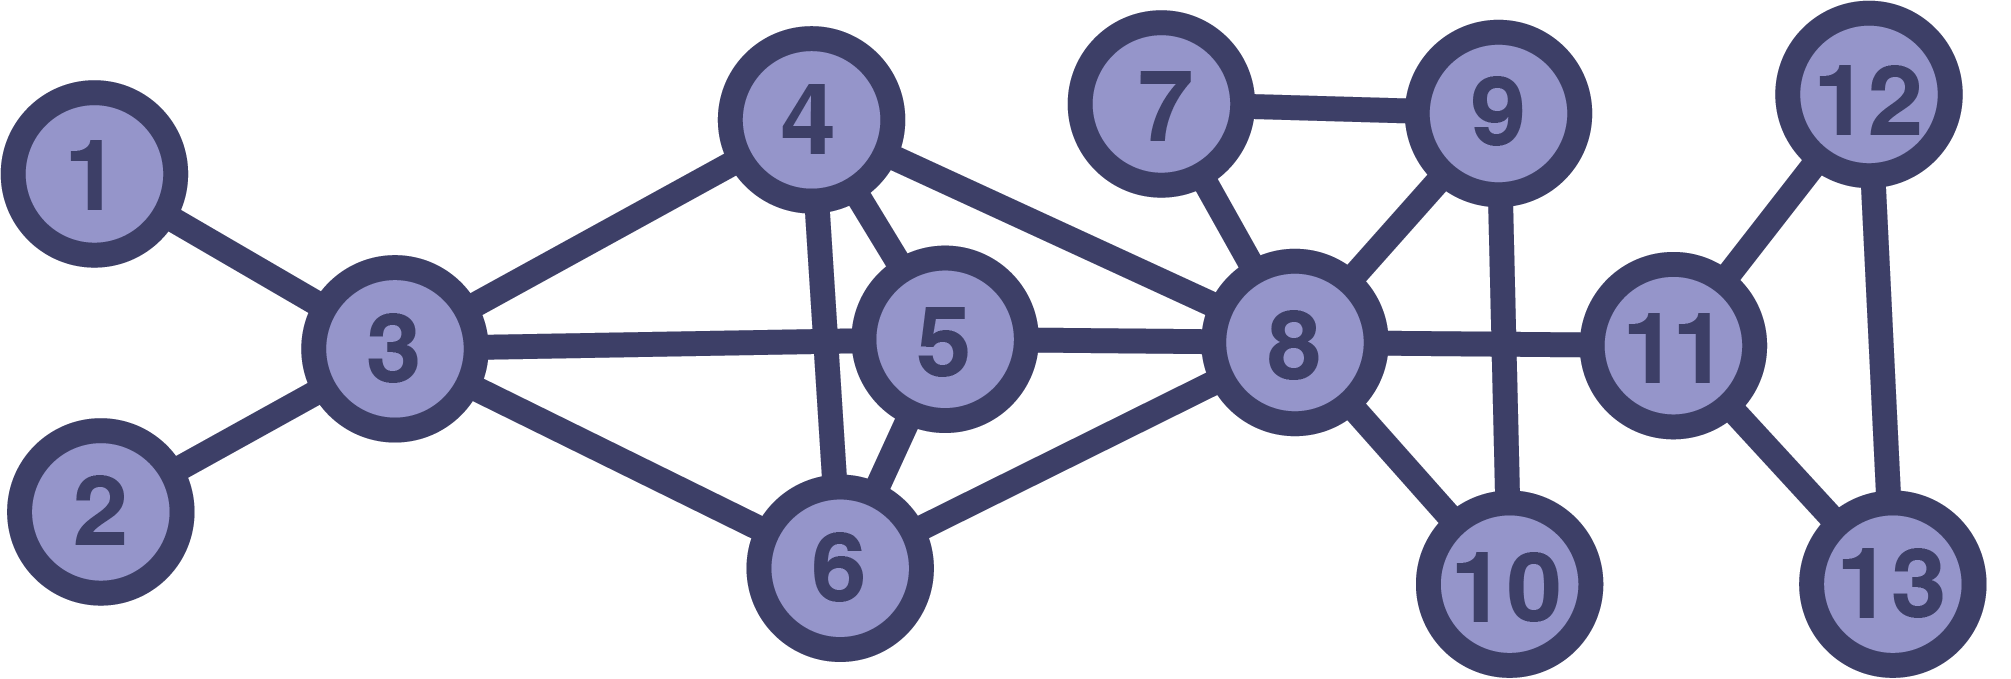
\includegraphics[width=0.75\textwidth]{symmetry}
\end{center}

\solution
Nodes 1 and 2 form a symmetry orbit. There should be a localized eigenvector. We can guess the eigenvector
\eq{
\vec{v_1} = (1,-1,0,0,0,0,0,0,0,0,0,0,0)^{\rm T} 
}
the corresponding eigenvalue is $\lambda_1=0$.

Furthermore, nodes 4, 5, 6 form a symmetric triangle. The eigenvectors can be assigned differently, but we can find two linearly independent localized eigenvectors. For example 
\eq{
\vec{v_2} = (0,0,0,1,-1,0,0,0,0,0,0,0,0)^{\rm T} 
}
\eq{
\vec{v_3} = (0,0,0,0,1,-1,0,0,0,0,0,0,0)^{\rm T} 
}
When we multiply either of these two vectors with the adjacency matrix the -1 and the 1 change places and everything else remains zero. SO the eigenvalues are $\lambda_2=\lambda_3=-1$.

Also 12 and 13 are symmetric which gives us the eigenvector 
\eq{
\vec{v_4} = (0,0,0,0,0,0,0,0,0,0,0,1,-1)^{\rm T} 
}
and another eigenvalue $\lambda_4=-1$. 

Finally, node 7 and 10 are another symmetric pair, their locvalized eigenvector is 
\eq{
\vec{v_5} = (0,0,0,0,0,0,1,0,0,-1,0,0,0)^{\rm T}
}
and the corresponding eigenvalue is $\lambda_5=0$.


